\documentclass[11pt,a4paper]{article}
% ── packages ──
\usepackage[utf8]{inputenc}
\usepackage[T1]{fontenc}
\usepackage{lmodern}
\usepackage[margin=2.2cm]{geometry}
\usepackage{graphicx}
\usepackage{xcolor}
\usepackage{booktabs}
\usepackage{tabularx}
\usepackage{longtable}
\usepackage{hyperref}
\usepackage{amsmath,amssymb}
\usepackage{enumitem}
\usepackage[most]{tcolorbox}
\usepackage{tikz}
\usetikzlibrary{shapes.geometric,arrows.meta,positioning,fit}
\usepackage{listings}

\hypersetup{colorlinks,linkcolor=blue!60!black,urlcolor=blue!70!black,
            citecolor=green!50!black}

% ── listing style ──
\definecolor{codebg}{HTML}{F5F5F5}
\definecolor{kw}{HTML}{0077AA}
\definecolor{str}{HTML}{DD4A22}
\definecolor{cmt}{HTML}{5C6370}
\lstset{
  language=Python,
  basicstyle=\ttfamily\footnotesize,
  backgroundcolor=\color{codebg},
  keywordstyle=\color{kw}\bfseries,
  stringstyle=\color{str},
  commentstyle=\color{cmt}\itshape,
  breaklines=true,
  frame=single,
  framesep=4pt,
  numbers=left,
  numberstyle=\tiny\color{gray},
  xleftmargin=1em,
  aboveskip=8pt,
  belowskip=8pt,
}

% ── custom boxes ──
\newtcolorbox{keybox}[1][]{colback=blue!5,colframe=blue!60!black,
  fonttitle=\bfseries,title=#1}
\newtcolorbox{physbox}[1][]{colback=green!5,colframe=green!50!black,
  fonttitle=\bfseries,title=#1}
\newtcolorbox{warnbox}[1][]{colback=red!5,colframe=red!60!black,
  fonttitle=\bfseries,title=#1}
\newtcolorbox{analogybox}[1][]{colback=yellow!8,colframe=orange!70!black,
  fonttitle=\bfseries,title=#1}

\title{
  \textbf{Code Walkthrough --- Explained Simply}\\[4pt]
  \Large Objective 1: Physics-Informed XAI OWTTransformer (v4)\\[2pt]
  \large \texttt{objective1\_XAI\_transformer\_demo.py}
}
\author{PFE Research Project}
\date{February 2026}

\begin{document}
\maketitle
\tableofcontents
\newpage


% ====================================================================
\section{What Does This Code Do?  (The Big Picture)}
% ====================================================================

\begin{keybox}[One-sentence summary]
This code \textbf{trains an AI model} that learns to predict how an
offshore wind turbine's foundation \textbf{weakens step by step}
during a typhoon --- and then \textbf{explains} which inputs mattered
most for each prediction.
\end{keybox}

\subsection{The Real-World Problem}

When a typhoon hits an offshore wind turbine (OWT), the repeated
pushing and pulling of waves and wind \textbf{degrades the soil}
around the pile foundation.  This makes the foundation softer
(lower stiffness), which changes how the tower vibrates (lower
natural frequency).  Engineers need to know:

\begin{itemize}[nosep]
  \item How much did the soil degrade?  ($G/G_{\max}$)
  \item How much did the foundation weaken?  ($H_t$)
  \item What is the new vibration frequency?  ($f_0$)
  \item \textbf{Why} did the model make that prediction?  (XAI)
\end{itemize}

\subsection{What Goes In and What Comes Out}

Think of the model as a \textbf{black box with 12 dials going in
and 7 gauges coming out}:

\begin{center}
\begin{tabular}{lll}
\toprule
\textbf{Role} & \textbf{What it is} & \textbf{How many numbers} \\
\midrule
\multicolumn{3}{l}{\textit{--- 12 Inputs (what we tell the model) ---}} \\
Pile length          & $L$ --- how long the pile is          & 1 \\
Pile diameter        & $D$ --- how wide the pile is          & 1 \\
Eccentricity         & $e$ --- offset of the load            & 1 \\
Previous stiffness   & $H_{t-1}$ --- how stiff it was last step & 3 \\
Previous mass        & $M_{t-1}$ --- how heavy it was        & 2 \\
Previous soil health & $G/G_{\max,t-1}$ --- soil quality last step & 1 \\
Previous frequency   & $f_{0,t-1}$ --- vibration freq.\ last step & 1 \\
Current displacement & $u_t$ --- how far it moved sideways   & 1 \\
Current rotation     & $\theta_t$ --- how much it tilted     & 1 \\
\midrule
\multicolumn{3}{l}{\textit{--- 7 Outputs (what the model predicts) ---}} \\
New stiffness     & $H_t$ --- 3 directions ($K_L, K_R, K_{LR}$)  & 3 \\
New mass          & $M_t$ --- lateral and rotational              & 2 \\
New soil health   & $G/G_{\max,t}$ --- how degraded the soil is  & 1 \\
New frequency     & $f_{0,t}$ --- the new vibration frequency     & 1 \\
\bottomrule
\end{tabular}
\end{center}

\begin{analogybox}[Everyday analogy]
Imagine a doctor checking a patient every hour during an illness.
Each hour, the doctor looks at \textbf{yesterday's blood test results}
(previous state) and \textbf{today's symptoms} (current loading),
then predicts \textbf{today's blood test results} (new state).
Our model does the same thing, but for a wind turbine foundation
during a typhoon.
\end{analogybox}

\subsection{Architecture Diagram}

\begin{center}
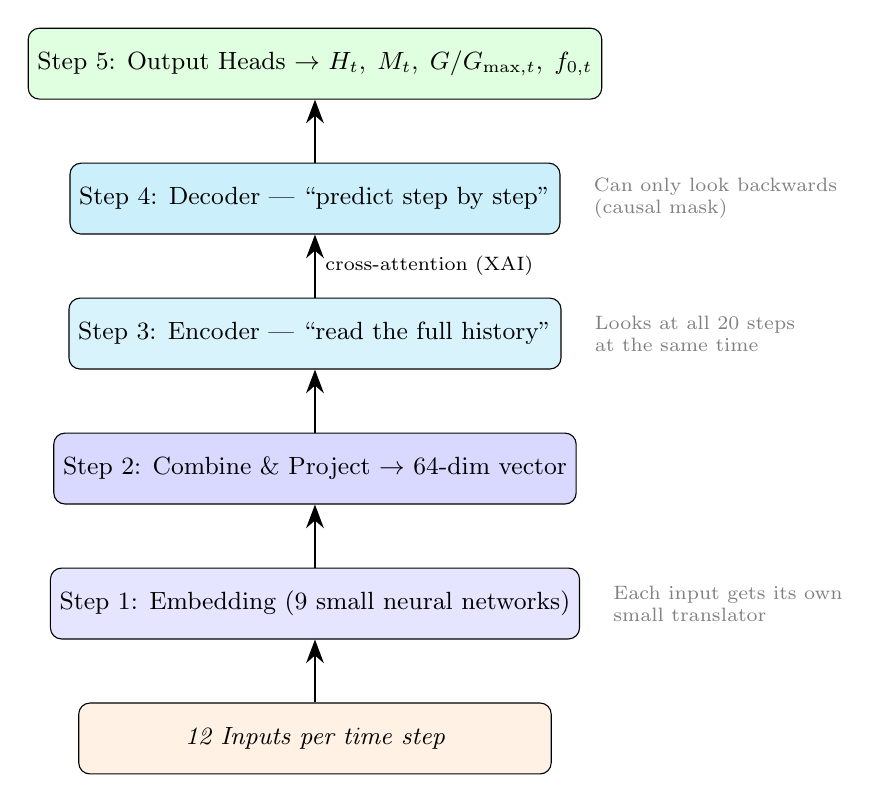
\begin{tikzpicture}[
  block/.style = {rectangle, draw, rounded corners, minimum width=6cm,
                  minimum height=0.9cm, align=center, font=\small},
  io/.style    = {rectangle, draw, rounded corners, minimum width=6cm,
                  minimum height=0.9cm, align=center, font=\small\itshape,
                  fill=orange!10},
  arr/.style   = {-{Stealth[length=3mm]}, thick},
  note/.style  = {font=\scriptsize\color{gray}, align=left},
  node distance = 0.8cm,
]
  \node[io]    (in)   {12 Inputs per time step};
  \node[block, above=of in,  fill=blue!10]   (emb)
    {Step 1: Embedding (9 small neural networks)};
  \node[block, above=of emb, fill=blue!15]   (ff)
    {Step 2: Combine \& Project $\to$ 64-dim vector};
  \node[block, above=of ff,  fill=cyan!15]   (enc)
    {Step 3: Encoder --- ``read the full history''};
  \node[block, above=of enc, fill=cyan!20]   (dec)
    {Step 4: Decoder --- ``predict step by step''};
  \node[block, above=of dec, fill=green!12]  (out)
    {Step 5: Output Heads $\to$ $H_t,\;M_t,\;G/G_{\max,t},\;f_{0,t}$};

  \draw[arr] (in)  -- (emb);
  \draw[arr] (emb) -- (ff);
  \draw[arr] (ff)  -- (enc);
  \draw[arr] (enc) -- (dec) node[midway,right,font=\scriptsize]{cross-attention (XAI)};
  \draw[arr] (dec) -- (out);

  \node[note, right=0.3cm of emb] {Each input gets its own\\small translator};
  \node[note, right=0.3cm of enc] {Looks at all 20 steps\\at the same time};
  \node[note, right=0.3cm of dec] {Can only look backwards\\(causal mask)};
\end{tikzpicture}
\end{center}


% ====================================================================
\section{The Code, Step by Step}
% ====================================================================

% --------------------------------------------------------------------
\subsection{Step 0: Settings (Lines 19--33)}
% --------------------------------------------------------------------

Before anything runs, we set the ``rules of the game'':

\begin{lstlisting}
N_SAMPLES, SEQ_LEN = 300, 20        # 300 scenarios, 20 steps each
D_MODEL, N_HEADS   = 64, 4          # brain size & attention heads
EPOCHS, BATCH, LR   = 80, 32, 1e-3  # 80 rounds, 32 at a time, speed 0.001
DOF, M_DIM          = 3, 2          # 3 stiffness + 2 mass values
\end{lstlisting}

\textbf{What this means in plain English:}
\begin{itemize}[nosep]
  \item We create \textbf{300 fake typhoon scenarios}, each with
        \textbf{20 time steps} (like 20 snapshots during the storm).
  \item The model's internal ``brain'' works with \textbf{64 numbers}
        at a time and uses \textbf{4 attention heads} (4 different ways
        of paying attention to the data simultaneously).
  \item We train for \textbf{80 rounds} (epochs), feeding
        \textbf{32 scenarios at a time} (batch), with a learning speed
        of \textbf{0.001} (small steps so the model learns carefully).
\end{itemize}

We also set the \textbf{loss weights} --- how much the model should
care about each rule:

\begin{lstlisting}
W = dict(H=1., M=1., G=1., f0=1.,   # care about matching the data
         freq=.5,                     # f0 must agree with physics formula
         monoH=.3, monoG=.3,         # stiffness & soil can only go DOWN
         pos=.3, Grange=.3)          # no negative values, G in [0,1]
\end{lstlisting}

\begin{analogybox}[Think of it like exam grading]
Matching the real data is worth \textbf{1 point each} (most important).
Following physics rules is worth \textbf{0.3--0.5 points} (still
important, but the model won't be punished as harshly if it's slightly
off on these).
\end{analogybox}


% --------------------------------------------------------------------
\subsection{Step 1: Creating Fake Data (Lines 36--101)}
% --------------------------------------------------------------------

Since we don't have real sensor data yet, we \textbf{generate synthetic
data} that follows the same physics a real turbine would.  The function
\texttt{make\_data()} does this:

\subsubsection{a) Pile Geometry (constant for each scenario)}

\begin{lstlisting}
L = torch.rand(N,1)*.8+.1   # pile length:   random in [0.1, 0.9]
D = torch.rand(N,1)*.8+.1   # pile diameter:  random in [0.1, 0.9]
e = torch.rand(N,1)*.6+.1   # eccentricity:   random in [0.1, 0.7]
\end{lstlisting}

These three numbers describe the \textbf{physical shape} of the pile.
They stay the same across all 20 time steps (the pile doesn't change
shape during a storm).

\subsubsection{b) Initial Conditions (before the typhoon starts)}

\begin{lstlisting}
H0 = (.3*D + .25*L + .15).expand(-1, DOF)  # initial stiffness
G0 = torch.ones(N)                          # soil health = 100%
f0_init = (.30*torch.sqrt((H0[:,1]/M0[:,1]  # initial frequency
           .clamp(min=.01)))).clamp(.1,.4)
\end{lstlisting}

\textbf{Key idea:}  Before the typhoon, the soil is \textbf{perfectly
healthy} ($G/G_{\max} = 1.0$), the stiffness is at its maximum, and
$f_0$ is calculated from the physics formula:
\[
  f_0 = 0.30 \times \sqrt{\frac{K_R}{M_{\text{rot}}}}
\]
This formula says: stiffer foundation $\to$ higher vibration frequency
(like a tighter guitar string vibrates faster).

\subsubsection{c) Simulating the Typhoon (20 steps)}

This is the heart of the data generation --- a \texttt{for} loop that
simulates what happens at each time step:

\begin{lstlisting}
for t in range(T):       # T = 20 time steps
    # How strong is the load right now?
    load = (u[:,t]**2 + th[:,t]**2).sqrt()

    # Soil degrades (gets weaker) with each push
    Gp = (Gp - .012*load - noise).clamp(.05, 1.)

    # Stiffness drops because the soil is weaker
    Hp = (Hp - (1 - ratio_drop)*Hp - noise).clamp(min=.01)

    # Natural frequency follows from physics
    f0_t = (.30*torch.sqrt((Hp[:,1]/Mp[:,1]))).clamp(.1,.4)
\end{lstlisting}

\textbf{What happens at each step:}
\begin{enumerate}[nosep]
  \item \textbf{Measure the load:} combine lateral push ($u$) and
        tilt ($\theta$) into one number.
  \item \textbf{Soil degrades:} $G/G_{\max}$ drops a little
        (bigger load $=$ bigger drop).  It can never go below 0.05.
  \item \textbf{Stiffness drops:} because the soil is weaker, the
        foundation gets softer.
  \item \textbf{Frequency updates:} softer foundation $=$ lower $f_0$.
\end{enumerate}

\begin{physbox}[The degradation chain]
This is the core physics our model must learn:
\[
  \underbrace{G/G_{\max} \downarrow}_{\text{soil degrades}}
  \;\longrightarrow\;
  \underbrace{K_R,\; K_L,\; K_{LR} \downarrow}_{\text{stiffness drops}}
  \;\longrightarrow\;
  \underbrace{f_0 \downarrow}_{\text{frequency shifts down}}
\]
\end{physbox}


% --------------------------------------------------------------------
\subsection{Step 2: Building the AI Model (Lines 103--243)}
% --------------------------------------------------------------------

This is the ``brain'' of the system --- the \textbf{OWTTransformer}.
Let's go through each part.

\subsubsection{a) Embedding: Translating Inputs into a Common Language}

Raw inputs have different scales and meanings (a length in meters
vs.\ a frequency in Hz).  The embedding layers \textbf{translate} each
input into a shared 16-number representation:

\begin{lstlisting}
self.embs = nn.ModuleList([
    nn.Linear(1, 16),      # L  (pile length)
    nn.Linear(1, 16),      # D  (pile diameter)
    nn.Linear(1, 16),      # e  (eccentricity)
    nn.Linear(DOF, 16),    # H_{t-1}  (prev stiffness, 3 values)
    nn.Linear(M_DIM, 16),  # M_{t-1}  (prev mass, 2 values)
    nn.Linear(1, 16),      # G/Gmax_{t-1}  (prev soil health)
    nn.Linear(1, 16),      # f0_{t-1}  (prev frequency)
    nn.Linear(1, 16),      # u_t  (lateral push)
    nn.Linear(1, 16),      # theta_t  (tilt)
])
\end{lstlisting}

Each \texttt{nn.Linear(in, 16)} is a tiny neural network with just
one layer.  It takes the raw number(s) and produces 16 numbers that
the transformer can work with.  Then all 9 embeddings are
\textbf{concatenated} ($9 \times 16 = 144$ numbers) and compressed
down to 64:

\begin{lstlisting}
self.proj = nn.Sequential(
    nn.Linear(9*16, 64),   # 144 -> 64
    nn.ReLU(),             # activation (keep positive values)
    nn.Linear(64, 64),     # refine
)
\end{lstlisting}

\begin{analogybox}[Translation analogy]
Imagine 9 people speaking different languages.  Each embedding is a
\textbf{personal translator} that converts their language into a
\textbf{common language} (64 numbers).  Now the transformer can
understand all of them.
\end{analogybox}

\subsubsection{b) Positional Encoding: Telling the Model ``What Time Is It?''}

A transformer processes all time steps at once, so it doesn't
naturally know which step came first.  We add a unique
\textbf{time stamp} to each step using sine and cosine waves:

\begin{lstlisting}
def sinusoidal_pe(length, d):
    pe[0, :, 0::2] = torch.sin(pos * div)   # even positions
    pe[0, :, 1::2] = torch.cos(pos * div)   # odd positions
    return pe
\end{lstlisting}

This is like writing ``Step 1'', ``Step 2'', \ldots, ``Step 20'' on
each input before handing it to the transformer.

\subsubsection{c) Encoder: Reading the Full History}

The encoder looks at \textbf{all 20 time steps simultaneously} and
figures out the relationships between them:

\begin{lstlisting}
enc_layer = nn.TransformerEncoderLayer(
    D_MODEL, N_HEADS, FF_DIM,   # 64-dim, 4 heads, 128-dim FFN
    dropout=.1, batch_first=True
)
self.encoder = nn.TransformerEncoder(enc_layer, N_LAYERS)  # 2 layers
\end{lstlisting}

\textbf{What it does:}  Using \textbf{self-attention}, each time step
``looks at'' every other time step and decides which ones are most
relevant.  For example, step~15 might pay a lot of attention to
step~14 (the immediate past) and step~1 (the initial condition).

Having \textbf{4 heads} means the encoder does this 4 different ways
simultaneously --- one head might focus on recent steps, another on
early steps, another on steps with high loading, etc.

\subsubsection{d) Decoder: Predicting Step by Step}

The decoder receives the encoder's summary and generates predictions
\textbf{one step at a time}, using a causal mask so that step~$t$
can only see steps $1, 2, \ldots, t$ (not the future):

\begin{lstlisting}
# Causal mask: prevents looking into the future
mask = nn.Transformer.generate_square_subsequent_mask(T)

# Self-attention (decoder looks at its own past predictions)
a, _ = self.dec_self(x, x, x, attn_mask=mask)
x = self.dec_norms[0](x + a)

# Cross-attention (decoder asks the encoder for help)
a, cw = self.dec_cross(x, memory, memory, need_weights=True)
self.cross_attn_w = cw.detach()   # SAVE for XAI!
x = self.dec_norms[1](x + a)

# Feed-forward (process the combined information)
x = self.dec_norms[2](x + self.dec_ffn(x))
\end{lstlisting}

\textbf{Three sub-steps:}
\begin{enumerate}[nosep]
  \item \textbf{Self-attention:}  The decoder looks at its own previous
        outputs (``what did I predict before?'').
  \item \textbf{Cross-attention:}  The decoder asks the encoder
        (``what does the full history say?'').  \textbf{This is the
        key XAI signal} --- we save these weights to see which inputs
        the model relied on.
  \item \textbf{Feed-forward:}  A simple neural network refines the
        combined information.
\end{enumerate}

\begin{analogybox}[Analogy: writing an essay]
The \textbf{encoder} is like reading the entire textbook (all 20 steps
at once).  The \textbf{decoder} is like writing the essay one sentence
at a time --- you can look back at what you already wrote
(self-attention) and check the textbook again (cross-attention), but
you can't peek at future sentences.
\end{analogybox}

\subsubsection{e) Output Heads: Four Separate Predictions}

After the decoder, four small neural networks each produce one type
of output:

\begin{lstlisting}
# Stiffness: must be positive -> Softplus activation
self.head_H = nn.Sequential(
    nn.Linear(64, 64), nn.ReLU(),
    nn.Linear(64, 3),  nn.Softplus()   # always > 0
)

# Mass: must be positive -> Softplus activation
self.head_M = nn.Sequential(
    nn.Linear(64, 64), nn.ReLU(),
    nn.Linear(64, 2),  nn.Softplus()   # always > 0
)

# Soil health: must be between 0 and 1 -> Sigmoid activation
self.head_G = nn.Sequential(
    nn.Linear(64, 32), nn.ReLU(),
    nn.Linear(32, 1),  nn.Sigmoid()    # always in [0, 1]
)

# Frequency: must be in [0.1, 0.4] Hz -> Scaled Sigmoid
self.head_f0 = nn.Sequential(
    nn.Linear(64, 32), nn.ReLU(),
    nn.Linear(32, 1)   # raw output
)
# Then in forward(): f0 = 0.1 + 0.3 * sigmoid(raw)
\end{lstlisting}

\begin{warnbox}[Why different activations for each output?]
Physics tells us what values are possible:
\begin{itemize}[nosep]
  \item \textbf{Stiffness \& mass} can never be negative $\to$
        \textbf{Softplus} (always $> 0$).
  \item \textbf{$G/G_{\max}$} is a ratio from 0\% to 100\% $\to$
        \textbf{Sigmoid} (always between 0 and 1).
  \item \textbf{$f_0$} for monopile OWTs ranges from 0.1 to 0.4~Hz $\to$
        \textbf{Scaled sigmoid}: $f_0 = 0.1 + 0.3 \times \sigma(\cdot)$,
        which maps any number into [0.1,\;0.4].
\end{itemize}
By choosing the right activation, we \textbf{build physics directly
into the architecture} --- the model literally \emph{cannot} output
impossible values.
\end{warnbox}


% --------------------------------------------------------------------
\subsection{Step 3: The Physics-Informed Loss Function (Lines 245--275)}
% --------------------------------------------------------------------

The loss function tells the model \textbf{how wrong it is}.
Unlike a standard AI that only checks ``did you match the data?'',
our loss has \textbf{9 terms} that also enforce physics:

\begin{lstlisting}
def physics_loss(Hp, Mp, Gp, fp, Ht, Mt, Gt, ft):
    # --- Data matching (did the model get close?) ---
    L_H  = F.mse_loss(Hp, Ht)    # stiffness error
    L_M  = F.mse_loss(Mp, Mt)    # mass error
    L_G  = F.mse_loss(Gp, Gt)    # G/Gmax error
    L_f0 = F.mse_loss(fp, ft)    # frequency error
\end{lstlisting}

These first 4 terms are \textbf{mean squared error} (MSE): they
measure how far the prediction ($Hp$) is from the truth ($Ht$),
square it (so big errors count more), and average.

\begin{lstlisting}
    # --- Physics rule: f0 must agree with the formula ---
    f0_phys = .30 * sqrt(K_R / M_rot)
    L_freq  = MSE(predicted_f0, f0_from_formula)
\end{lstlisting}

This is \textbf{Law of Thermodynamics \#1} (LoT1): the predicted
frequency must be \textbf{consistent} with the predicted stiffness
and mass.  If the model predicts high stiffness but low frequency,
this penalty kicks in.

\begin{lstlisting}
    # --- Physics rule: things can only get worse ---
    L_monoH = penalty if stiffness goes UP between steps
    L_monoG = penalty if G/Gmax goes UP between steps
\end{lstlisting}

This is \textbf{Law of Thermodynamics \#2} (LoT2): during a typhoon,
the soil only degrades --- it doesn't magically heal.  If the model
predicts that stiffness \emph{increased} from step~5 to step~6,
it gets penalized.

\begin{lstlisting}
    # --- Physical bounds ---
    L_pos    = penalty if stiffness or mass < 0
    L_Grange = penalty if G/Gmax outside [0, 1]
\end{lstlisting}

These are \textbf{sanity checks}: stiffness and mass cannot be
negative, and $G/G_{\max}$ (a ratio) must stay between 0 and 1.

Finally, everything is added up with weights:

\begin{lstlisting}
    total = 1.0*L_H + 1.0*L_M + 1.0*L_G + 1.0*L_f0
          + 0.5*L_freq
          + 0.3*L_monoH + 0.3*L_monoG
          + 0.3*L_pos + 0.3*L_Grange
\end{lstlisting}

\begin{center}
\small
\begin{tabular}{llp{5.5cm}l}
\toprule
\textbf{\#} & \textbf{Loss term} & \textbf{What it checks} & \textbf{Weight} \\
\midrule
1 & $\mathcal{L}_H$    & Stiffness matches data     & 1.0 \\
2 & $\mathcal{L}_M$    & Mass matches data           & 1.0 \\
3 & $\mathcal{L}_G$    & $G/G_{\max}$ matches data   & 1.0 \\
4 & $\mathcal{L}_{f_0}$& Frequency matches data      & 1.0 \\
\midrule
5 & $\mathcal{L}_{\text{freq}}$ & $f_0$ agrees with
    $0.30\sqrt{K_R/M_{\text{rot}}}$ & 0.5 \\
6 & $\mathcal{L}_{\text{monoH}}$ & Stiffness never increases & 0.3 \\
7 & $\mathcal{L}_{\text{monoG}}$ & $G/G_{\max}$ never increases & 0.3 \\
8 & $\mathcal{L}_{\text{pos}}$ & No negative stiffness/mass & 0.3 \\
9 & $\mathcal{L}_{G\text{range}}$ & $G/G_{\max} \in [0,1]$ & 0.3 \\
\bottomrule
\end{tabular}
\end{center}


% --------------------------------------------------------------------
\subsection{Step 4: Preparing the Data for Training (Lines 277--296)}
% --------------------------------------------------------------------

The model is \textbf{autoregressive}: at each step, it receives the
\textbf{previous step's answer} as input.  During training, we use
the \textbf{real} previous answer (not the model's guess) --- this
is called \textbf{teacher forcing}.

\begin{lstlisting}
def make_batch(data, idx):
    H, M, G, f0 = data['H'][idx], ...
    # Shift right: prepend initial value, drop last step
    H_prev = cat([H0, H[:, :-1]])   # [H0, H1, ..., H18]
    #              targets are:       [H1, H2, ..., H19]
    ...
\end{lstlisting}

\textbf{Visual example for $G/G_{\max}$:}

\begin{center}
\begin{tabular}{lcccccc}
\toprule
           & Step 0 & Step 1 & Step 2 & $\cdots$ & Step 19 \\
\midrule
\textbf{Input}  (prev) & $G_0{=}1.0$ & $G_1$ & $G_2$ & $\cdots$ & $G_{18}$ \\
\textbf{Target} (true) & $G_1$       & $G_2$ & $G_3$ & $\cdots$ & $G_{19}$ \\
\bottomrule
\end{tabular}
\end{center}

So the model always sees ``yesterday's'' value and tries to predict
``today's'' value.


% --------------------------------------------------------------------
\subsection{Step 5: Training the Model (Lines 298--355)}
% --------------------------------------------------------------------

Training is the process of \textbf{showing the model examples and
correcting its mistakes} --- repeated 80 times (epochs):

\begin{lstlisting}
for ep in range(80):            # 80 rounds of training
    perm = torch.randperm(n_tr) # shuffle the 255 training scenarios
    for i in range(0, 255, 32): # process 32 at a time (mini-batch)
        # 1. Forward pass: give inputs, get predictions
        Hp, Mp, Gp, fp = model(inputs)

        # 2. Compute loss: how wrong was the model? (9 terms)
        loss = physics_loss(predictions, targets)

        # 3. Backpropagation: figure out which weights to adjust
        loss.backward()

        # 4. Clip gradients: prevent wild jumps
        clip_grad_norm_(model.parameters(), 1.0)

        # 5. Update weights: make the model slightly better
        optimizer.step()
\end{lstlisting}

\begin{analogybox}[Training analogy]
Training is like a student doing \textbf{80 rounds of practice exams}.
Each round:
\begin{enumerate}[nosep]
  \item The student tries to answer (\textbf{forward pass}).
  \item The teacher marks the exam (\textbf{loss function}).
  \item The student studies their mistakes (\textbf{backpropagation}).
  \item The student updates their notes (\textbf{weight update}).
\end{enumerate}
After 80 rounds, the student (model) should be quite good!
\end{analogybox}

\textbf{Additional training tricks:}
\begin{itemize}[nosep]
  \item \textbf{Adam optimizer}: a smart algorithm that adjusts the
        learning speed for each weight individually.
  \item \textbf{Cosine annealing}: the learning rate starts at 0.001
        and slowly decreases to near-zero (big steps early,
        fine-tuning later).
  \item \textbf{Gradient clipping}: if any weight wants to change too
        dramatically, we cap it at 1.0 to keep training stable.
\end{itemize}


% --------------------------------------------------------------------
\subsection{Step 6: Testing and Evaluation (Lines 339--355)}
% --------------------------------------------------------------------

After training, we test on the \textbf{15\% of data the model has
never seen} (45 scenarios):

\begin{lstlisting}
model.eval()                # disable dropout (no randomness)
with torch.no_grad():       # don't compute gradients (faster)
    Hp, Mp, Gp, fp = model(test_inputs)
    # For each output, print:
    for name, pred, true in [("H",...), ("M",...), ...]:
        print(f"  MSE={...}  R^2={...}  MAPE={...}%")
\end{lstlisting}

Three metrics are reported:
\begin{itemize}[nosep]
  \item \textbf{MSE} (Mean Squared Error): average of (prediction
        $-$ truth)$^2$.  Lower is better.  Zero means perfect.
  \item \textbf{$R^2$} (R-squared): how much of the variation the
        model explains.  \textbf{1.0 = perfect}, 0 = no better than
        guessing the average, negative = terrible.
  \item \textbf{MAPE} (Mean Absolute Percentage Error): average \%
        error.  \textbf{Lower is better}.
\end{itemize}


% --------------------------------------------------------------------
\subsection{Step 7: Visualization --- The 10-Panel Figure (Lines 357--end)}
% --------------------------------------------------------------------

The code generates one large figure with 10 panels, saved as
\texttt{objective1\_XAI\_results.png}:

\begin{center}
\small
\begin{tabular}{cp{9cm}}
\toprule
\textbf{Panel} & \textbf{What it shows} \\
\midrule
(a) & \textbf{Training losses over 80 epochs} (log scale).
      All 8 loss components should decrease.  If they plateau,
      training is done. \\
(b) & \textbf{$K_L$ (lateral stiffness):} circles = truth,
      squares = prediction, for 4 test scenarios. \\
(c) & Same as (b) but for \textbf{$K_R$} (rotational stiffness). \\
(d) & Same for \textbf{$M_{\text{rot}}$} (rotational mass). \\
(e) & \textbf{$G/G_{\max}$:} soil degradation over 20 steps.
      Should decrease from $\sim$1.0 toward 0. \\
(f) & \textbf{$f_0$:} natural frequency over 20 steps.
      Should decrease as stiffness drops. \\
(g) & All \textbf{3 stiffness components} ($K_L, K_R, K_{LR}$)
      for one scenario, showing the degradation curves. \\
(h) & \textbf{$G/G_{\max}$} curve for one scenario:
      true vs.\ predicted, zoomed in. \\
(i) & \textbf{Cross-attention heatmap} (XAI): a colour grid showing
      which encoder time steps the decoder paid attention to.
      Bright red = high attention, blue = low. \\
(j) & \textbf{Attribution bar chart} (XAI): average attention per
      time step.  Taller bar = that step's inputs influenced the
      predictions more. \\
\bottomrule
\end{tabular}
\end{center}

\begin{keybox}[Panels (i) and (j) are the ``XAI'' --- Explainability]
Most AI models are ``black boxes'' --- you get a number but don't know
why.  Panels (i) and (j) \textbf{open the black box}:
\begin{itemize}[nosep]
  \item \textbf{(i) Cross-attention heatmap:}  Shows that when
        predicting step~15, the model looked mostly at
        steps~13--15 (recent history) and step~1 (initial condition).
  \item \textbf{(j) Attribution bars:}  Shows the \emph{average}
        importance of each step across all predictions.
\end{itemize}
This is critical for engineers: if the model says $f_0$ dropped,
they can see \emph{which time steps caused that prediction}.
\end{keybox}


% ====================================================================
\section{How Everything Connects}
% ====================================================================

\begin{center}
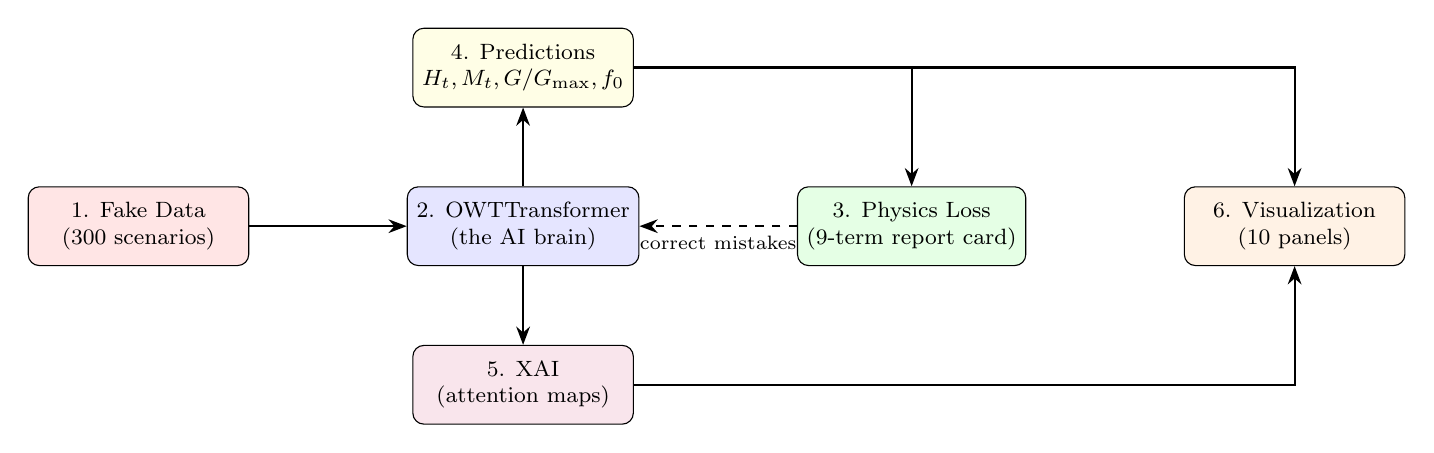
\begin{tikzpicture}[
  box/.style={rectangle, draw, rounded corners, minimum height=1cm,
              minimum width=2.8cm, align=center, font=\footnotesize},
  arr/.style={-{Stealth}, thick},
  node distance=1.5cm and 2cm,
]
  \node[box, fill=red!10]    (data)  {1. Fake Data\\(300 scenarios)};
  \node[box, fill=blue!10,  right=of data]  (model) {2. OWTTransformer\\(the AI brain)};
  \node[box, fill=green!10, right=of model] (loss)  {3. Physics Loss\\(9-term report card)};
  \node[box, fill=yellow!10, above=1cm of model] (out) {4. Predictions\\$H_t, M_t, G/G_{\max}, f_0$};
  \node[box, fill=purple!10, below=1cm of model] (xai) {5. XAI\\(attention maps)};
  \node[box, fill=orange!10, right=of loss] (viz) {6. Visualization\\(10 panels)};

  \draw[arr] (data) -- (model);
  \draw[arr] (model) -- (out);
  \draw[arr] (out.east) -| (loss);
  \draw[arr, dashed] (loss) -- node[below,font=\scriptsize]{correct mistakes} (model);
  \draw[arr] (model) -- (xai);
  \draw[arr] (out) -| (viz);
  \draw[arr] (xai) -| (viz);
\end{tikzpicture}
\end{center}


% ====================================================================
\section{Literature Positioning: What Exists vs.\ What Is New}
% ====================================================================

\subsection{What Already Exists}

\begin{center}
\small
\begin{tabularx}{\textwidth}{lXl}
\toprule
\textbf{Idea} & \textbf{Who did it} & \textbf{Reference} \\
\midrule
$G/G_{\max}$ curves & Lab experiments on soil degradation &
  Vucetic \& Dobry (1991) \\
Stiffness model & $H(t) = H_0 - \sum w_n H_n$ (TIM) &
  Gorini (2022, 2025) \\
Transformer & Encoder--decoder with attention for sequences &
  Vaswani et al.\ (2017) \\
$f_0 \propto \sqrt{K_R}$ & Natural frequency formula for monopiles &
  Bhattacharya (2019) \\
Attention roll-out & Multiplying attention maps for explainability &
  Abnar \& Zuidema (2020) \\
Physics-informed NN & Adding physics equations to the loss &
  Raissi et al.\ (2019) \\
\bottomrule
\end{tabularx}
\end{center}

\subsection{What Is New (Our Contribution)}

\begin{center}
\small
\begin{tabularx}{\textwidth}{lX}
\toprule
\textbf{Novelty} & \textbf{Why nobody did this before} \\
\midrule
$G/G_{\max}$ as both input \& output &
  Previous works either measure it or predict it --- we do both
  (autoregressive) inside a transformer \\
$f_0$ as both input \& output &
  Usually $f_0$ is calculated after the fact; here the model
  predicts it and feeds it back \\
Full chain $G/G_{\max} \to H \to f_0$ &
  No single model predicts the entire degradation chain with
  physics constraints \\
9-term physics loss &
  Combines data fitting + energy (LoT1) + dissipation (LoT2) +
  range constraints in one loss \\
Attention-based XAI for OWT &
  Using cross-attention weights to explain \emph{which load steps}
  caused the predicted degradation \\
\bottomrule
\end{tabularx}
\end{center}

\begin{physbox}[Novelty summary]
\textbf{No published paper} combines all five: (1)~$G/G_{\max}$ as
autoregressive I/O, (2)~coupled stiffness + frequency prediction,
(3)~thermodynamic physics constraints (LoT1 + LoT2), (4)~$G/G_{\max}$
range enforcement, and (5)~attention-based explainability --- all in
one transformer for post-typhoon OWT assessment.
\end{physbox}


% ====================================================================
\section{Quick Reference}
% ====================================================================

\begin{center}
\begin{tabular}{lp{8cm}}
\toprule
\textbf{File} & \textbf{What it is} \\
\midrule
\texttt{objective1\_XAI\_transformer\_demo.py} & The full runnable
  Python code ($\sim$460 lines) \\
\texttt{objective1\_XAI\_results.png} & The 10-panel output figure
  (generated automatically) \\
\bottomrule
\end{tabular}
\end{center}

\textbf{How to run:}
\begin{lstlisting}[language=bash]
C:/Users/youss/Downloads/PFE/.venv/Scripts/python.exe objective1_XAI_transformer_demo.py
\end{lstlisting}


% ====================================================================
\section{Glossary}
% ====================================================================

\begin{center}
\begin{tabular}{lp{9.5cm}}
\toprule
\textbf{Term} & \textbf{Plain-English Definition} \\
\midrule
$G/G_{\max}$ & Soil health ratio.  1.0 = perfectly healthy,
  0 = completely degraded.  Drops during a typhoon. \\
$H_t$   & Foundation stiffness at step $t$.  Three numbers
  ($K_L$, $K_R$, $K_{LR}$) describing how the pile resists
  lateral, rotational, and coupled forces. \\
$M_t$   & Foundation mass at step $t$.  Two numbers
  ($M_{\text{lat}}$, $M_{\text{rot}}$). \\
$f_0$   & Natural frequency --- the rate at which the turbine
  ``wants'' to vibrate (in Hz).  Lower = more dangerous. \\
Transformer & A type of AI that processes sequences by
  ``paying attention'' to different parts of the input. \\
Encoder  & Part of the transformer that reads the full input
  history at once. \\
Decoder  & Part that generates predictions step by step,
  only looking backwards. \\
Attention & A mechanism that lets the model decide which parts
  of the input are most relevant for each prediction. \\
XAI      & Explainable AI --- techniques that show \emph{why}
  the model made a prediction. \\
LoT1     & First Law of Thermodynamics: energy conservation.
  Here: $f_0$ must match $\sqrt{K_R/M_{\text{rot}}}$. \\
LoT2     & Second Law: things degrade, they don't spontaneously
  heal.  Stiffness and $G/G_{\max}$ can only go down. \\
MSE      & Mean Squared Error: average (prediction $-$ truth)$^2$. \\
$R^2$    & R-squared: 1.0 = perfect predictions,
  0 = as good as guessing the average. \\
MAPE     & Mean Absolute Percentage Error: average \% mistake. \\
Epoch    & One full pass through all training data. \\
Batch    & A small group of examples processed together
  (32 in our case). \\
OWT      & Offshore Wind Turbine. \\
TIM      & Thermodynamics-based Interface Model (Gorini 2025). \\
\bottomrule
\end{tabular}
\end{center}

\end{document}
